
%https://wstein.org/edu/2007/spring/ent/ent-html/node89.html
\Section{Elliptic-curve cryptography \& ECDSA}\label{ecdsa}
As covered in the introduction, Elliptic-curve cryptography (\textbf{ECC}) and ECDSA is a fundamental building block of bitcoin. Elliptic curve cryptography relies on intractability of calculating the discrete logarithm of a elliptic curve element with respect to a publicly known base point. Or put another way: It is easy to calculate elliptic curve multiplication with multiplicand $n$. But calculating $n$ from the resulting point is considered infeasible with sufficiently large curves and multiplicands.

%Not sure about the field
An elliptic curve is defined by the equation $Y^2=x^3+ax+b$ and six domain parameters $E(p,a,b,G,n,h)$. $\textbf{p}$ is the field that the curve is defined over, this is usually a very large prime number. The curve being defined over a field simply means that the points on the curve fall within $[0, p]$ rather than within the real numbers $\mathbb{R}$. In other words the curve is defined over the field $\mathbb{F}_{p}$. $\textbf{a}$ and $\textbf{b}$ are whatever number you put into the equation. $\textbf{G}$ is the generator point, that is the point on the curve that will be used in point multiplication later. $\textbf{n}$ is the order of G. What that means is that $n$ is the largest number that $G$ can be multiplied by before a point at infinity is produced. $n$ pretty much tells you the limit on how points on the curve that can be generated from $G$. $\textbf{h}$ is the co-factor of the curve. It can be calculated as follows: $h=\frac{1}{n}|(E(\mathbb{F}_{p})|$, where $|(E(\mathbb{F}_{p})|$ is the order/cardinality of the group of points possible on the curve over field $\mathbb{F}_{p}$. $n$ is derived from $G$, $G$ and $p$ should be chosen in such a way that $h \leq 4$, preferably $h=1$.

These domain parameters can be chosen manually or you can use predefined parameters. Elliptic curves that used predefined domain parameters are called named-curves. The named curve used by Bitcoin is called \texttt{Secp256k1}

\Subsection{Secp256k1}
\texttt{Secp256k1} is defined with the following domain parameters (hexadecimal):\\\\
$p=\texttt{FFFFFFFF FFFFFFFF FFFFFFFF FFFFFFFF FFFFFFFF FFFFFFFF FFFFFFFE FFFFFC2F}$\\
or alternatively:\\
$p=2^{256}-2^{32}-2^{9}-2^{8}-2^{7}-2^{6}-2^{4}-1$

$a=0$\\
$b=7$

$G=(\texttt{79BE667E F9DCBBAC 55A06295 CE870B07 029BFCDB 2DCE28D9 59F2815B 16F81798},\\ \null\qquad\:\:\: \texttt{483ADA77 26A3C465 5DA4FBFC 0E1108A8 FD17B448 A6855419 9C47D08F FB10D4B8})$


$n=\texttt{FFFFFFFF FFFFFFFF FFFFFFFF FFFFFFFE BAAEDCE6 AF48A03B BFD25E8C D0364141}$
$h=\texttt{1}$

\Subsection{Math on the elliptic curve}
Two mathematical operations needs to be defined to operate on the elliptic curve: addition and multiplication

\Subsubsection{Point addition}
Let's say you have to distinct points P and Q that both fall on curve $E(p,a,b,G,n,h)$ ($Y^2=x^3+ax+b$). 

$$P+Q=R \Rightarrow (X_P, Y_P) + (X_Q, Y_Q) = (X_R, Y_R)$$

$$X_R = \lambda^2-X_P-X_Q$$
$$Y_R = \lambda(x_P-X_R) -Y_P$$

where $\lambda$:

$$\lambda = \frac{Y_Q-Y_P}{X_Q - X_P} \mod p$$

\Subsubsection{Point multiplication}
If P and Q are coincident, meaning that they have the same coordinates the equation is slightly different. 

$$P+Q=R \Rightarrow P+P=R \Rightarrow 2P=R$$ 

This could be seen as P being multiplied with scalar 2. Most of the equation is the same as with addition, the difference is that:\\
$$\lambda = \frac{(3X^2_P + a)}{(2Y_P)} \mod p$$

\Subsubsection{Faster multiplication with large scalars}
Take $xP=R$ that could be calculated by summing P x times:
$$\sum_{n=1}^{x} P = R$$
This might work fine for smaller numbers but for a very large number, like $x=2^{100}$ it will take infeasible amount of time to calculate. Luckily there is a convenient short cut that you can take called double and add. 

First remember that: $P+P = 2P \Rightarrow 2P + P = 3P \Rightarrow 4P = 2(2P) \Rightarrow 8P = 2(2(2P))$

Lets say $x=200$ in binary terms this could be written as $x=128+64+8$ or $x=2^7+2^6+2^3$ thus $200P=R$ could be written as $$2^7P+2^6P+2^3P=R$$ which could be shorten to: $$2(2(2(2(2(2(2P)))))) + 2(2(2(2(2(2P))))) + 2(2(2P))$$ which looks cumbersome but now instead of 200 calculations you only have to do 18.


\Subsection{Private and public key}
Just as \texttt{RSA} cryptography, ECC relies on public-private key encryption and signatures. The public key can be shared freely to everyone, while the private key should, as the name implies, be kept private. Each unique private key has a corresponding public key, through mathematics it can be proven that someone holds the private key paired with a certain public key, without actually revealing the private key. 

In ECC \textbf{a private key is a really large number}. Imagine you have curve $E(p,a,b,G,n,h)$ and you want to generate a brand new private key k. k could be any number between 0 and $n$. Any $k > n$ will produce the exact same public key so that will not work. \textbf{A public key in ECC is represented by a point in 2D space}, more specifically a point that falls on the curve. To generate a public key P from a private key k you perform $kG = P$ as described in the section above.\\\\\\

\Subsubsection{Compressed key}
\begin{wrapfigure}{r}{0.3\textwidth}
	\begin{center}
		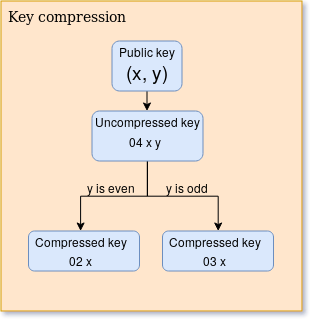
\includegraphics[width=0.4\textwidth]{background/images/key_compression.png}
	\end{center}
	\caption{How to compress the public key in ecc}
\end{wrapfigure}

The public key is quite large, with two 256-bit numbers representing coordinates. But there is a clever trick we can use to compress the size of the key. Take the \texttt{Secp256k1} curve for example ($Y^2=x^3+ax+b$). It is mirrored around the x-axis, meaning that for each x value there are two possible y values. Thus a public key can be represented by only it's x value plus a prefix telling you which resulting y-value to choose. 

Note that because y and x is over $\mathbb{F}_{p}$ there is no negative value, instead the y value is referred to as even or odd. 

\Subsection{ECDSA}
The main usage of ECC in cryptocurrency 
